\documentclass[a4paper, openright, twoside,11pt]{article}
\usepackage[utf8]{inputenc}
\usepackage[polish]{babel}

\usepackage[T1]{fontenc}
    \usepackage{float}
    \usepackage[backend=biber, style=alphabetic, sorting=ynt]{biblatex}
    \addbibresource{biblio.bib}

    \usepackage{graphicx}
    \usepackage{romannum}
    \usepackage{amsmath}
    \usepackage{mathtools}
    \usepackage{siunitx}
    \usepackage{gensymb}
    \usepackage{amssymb}
    
    \usepackage{hyperref}
    
    \usepackage{scrlayer}
    \DeclareNewLayer[
        foreground,
        %textarea,% use only the textarea
        contents={%
          \parbox[b][\layerheight][c]{\layerwidth}
            {\centering}%
        }
      ]{blankpage.fg}
    \DeclarePageStyleByLayers{blank}{blankpage.fg}
    
    
    
    \usepackage{listings}
    \usepackage{xcolor}
    \hypersetup{
        colorlinks=false,
        pdfborder={0 0 0},
    }
    
    \usepackage{comment}
    \usepackage[normalem]{ulem}
  
   
    \usepackage[margin=1.0in]{geometry}

    
    \usepackage{fancyhdr}
    \pagestyle{fancy}
    \fancyhf{}
    \lhead{Sztuczna Inteligencja}
    \rhead{Politechnika Rzeszowska}
    \cfoot{Strona \thepage}
    %\pagenumbering{arabic}
    
    \renewcommand{\lstlistlistingname}{Spis listingów}
    \setlength\parindent{0pt}



\begin{document}
\begin{titlepage}
            \begin{minipage}{0.3\linewidth}
                %\begin{flushleft}
                    
\includegraphics[width=1\columnwidth]{Grafika/prz_pl.png}
                %\end{flushleft}
            \end{minipage}
            \begin{minipage}{0.7\linewidth}
                \begin{center}
                    \large{Politechnika Rzeszowska\\
                    Wydział Elektrotechniki i Informatyki\\}
                    \Large\textbf{Katedra Informatyki i Automatyki}\\
                \end{center}
            \end{minipage}

            \begin{center}

                \vfill
                    \Huge Sztuczna Inteligencja\\[2cm]
                    \huge Projekt\\[2cm]
                    \huge Realizacja sieci neuronowej uczonej algorytmem wstecznej propagacji błędu z przyśpieszeniem metodą adaptacyjnego współczynnika uczenia uczącą się rozpoznawania rodzaju naczyń szklanych\\
                \vfill
            \end{center}



            
            
            \mbox{}
            \vfill
            \begin{flushright}
               \large{\textbf{Wykonał: \\}
               Artur Przystaś\\
               156321\\
                \Romannum{2} EF-DI\\[1cm]}
            \end{flushright}
            \begin{center}
                \large Rzeszów 2019
            \end{center}
        \end{titlepage}
        
    
    \newpage\null\thispagestyle{blank}\newpage
    \tableofcontents    
    \thispagestyle{empty}
    \newpage\null\thispagestyle{blank}
    
    \newpage
    
    \pagenumbering{arabic}
    \newpage
    \setcounter{page}{5}
    
    
    \section{Opis problemu}
    \subsection{Cel projektu}
    Celem projektu jest opracowanie i zrealizowanie sieci neuronowej uczonej algorytmem wstecznej propagacji błędu z przyśpieszeniem metodą adaptacyjnego współczynnika uczenia. Sieć neuronowa ma za zadnie zidentyfikować rodzaj naczyń szklanych. Problem został rozwiązany w programie Matlab R2019a, przy użyciu funkcji traingda.
    Prace obejmowały opracowanie wstępu teoretycznego, przygotowanie skryptu wielowarstwowej sieci neuronowej, przeprowadzenie eksperymentów, opracowanie na ich podstawie danych i wniosków. 

    \subsection{Opis danych}
    Sieć ma za zadnie identyfikować rodzaj naczyń szklanych za pomocą informacji o:
    
    \begin{enumerate}
        \item Współczynniku załamania
        \item Procentowej zawartości tlenku:
             \begin{itemize}
             \item sodu,
             \item magnezu,
            \item glinu,
            \item krzemu,
            \item potasu,
            \item wapnia
            \item baru,
            \item żelaza
            \end{itemize}
        \end{enumerate}
        
        
    Naczynia mogą należeć do następujących klas:
    \begin{enumerate}
        \item Szyba okienna poddana procesowi float
        \item Szyba okienna nie poddana procesowi float
        \item Szyba samochodowa poddana procesowi float
        \item Szyba samochodowa nie poddana procesowi float
        \item Pojemnik
        \item Zastawa stołowa
        \item Reflektor
    \end{enumerate}
    
    Dostarczone dane posiadają 219 przypadków. Ich dystrybucja wygląda następująco:
    \begin{enumerate}
        \item Szyby 163
            \begin{enumerate}
                \item Poddane procesowi float
                \begin{enumerate}
                    \item Szyby okienne: 70
                    \item Szyby samochodowe: 17
                \end{enumerate}
                \item Nie poddane procesowi float: 76 
                \begin{enumerate}
                    \item Szyby okienne: 76
                    \item Szyby samochodowe: 0
                \end{enumerate}
            \end{enumerate}
            \item Pozostałe
            \begin{enumerate}
                \item Pojemniki: 13
                \item Zastawy stołowe: 9
                \item Reflektory: 29
            \end{enumerate}
    \end{enumerate}
    Otrzymane dane zostały, w czasie wykonywania ćwiczenia, poddane normalizacji, tak by wartości znajdowały się w przedziale [-1;1].
    \clearpage
    \section{Zagadnienia teoretyczne}
    \subsection{Sieć neuronowa}
    Sieć neuronowa jest oparta na strukturze matematycznej i programowym, bądź sprzętowym modelu realizującym obliczenia przez warstwy sztucznych neuronów. Wykonują one obliczenia na wejściu a następnie przekazują te informacje do kolejnego neuronu tworząc sieć. Pierwowzorem sieci neuronowej jest ludzki mózg. 
    
    \subsection{Model neuronu}
    \begin{figure}[h]
        \centering
        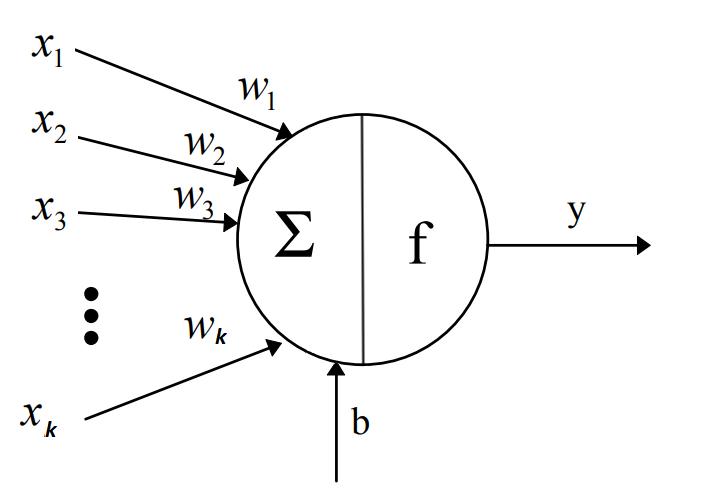
\includegraphics[width=0.6\textwidth]{Grafika/neuron.png}
        \caption{Model neuronu}
        \label{fig:neuron}
    \end{figure}
    
    Neuron to podstawowy element sieci neuronowej. Odpowiada on za przetwarzanie i przesyłanie danych do kolejnych neuronów. Jego elementy to:\\[0.1cm]
    $x_k$ - sygnały wejściowe\\
    $w_k$ - wagi wejść\\
    $y$ - wyjście\\
    $b$ - przesuniecie (bias)\\
    $f$ - funkcja aktywacji\\
    $k$ - liczba wejść\\
    \\[0.5cm]
    Sygnał wyjściowy neuronu y jest określony zależnością:
    \begin{equation} \label{funkcja aktywacji}
    y = f(\sum_{i=1}^k w_i x_i + b)
    \end{equation}
    
    Ponieważ do wyznaczenia wartości wyjścia $y$ służy wzór:
    \begin{equation}\label{fun_aktywacji}
    %y = f\left( \sum_{i=1}^k w_i x_i + b \right)
    y = f(n)
    \end{equation}
    
    Gdzie
    \begin{equation} \label{pobudzenieNeuronu}
    n = \sum_{i=1}^k w_i x_i + b
    \end{equation}
    
    Oznacza to, że sygnały wejściowe są mnożone przez swoje wagi, później sumowane. Otrzymana suma wraz z wartością biasu jest wejściem funkcji aktywacji, która zwraca wartość wyjściową neuronu.
    
    \subsection{Funkcja aktywacji}
    Odpowiedzialna jest za obliczenie sygnału wyjściowego neuronu. Różne funkcje są stosowane jako funkcje aktywacji, w zależności od potrzeb danej sieci neuronowej.
    W opracowanej sieci neuronowej zastosowane zostały funkcja sigmoidalna dla warstwy pierwszej i drugiej\\
    \begin{figure}[h]
        \centering
        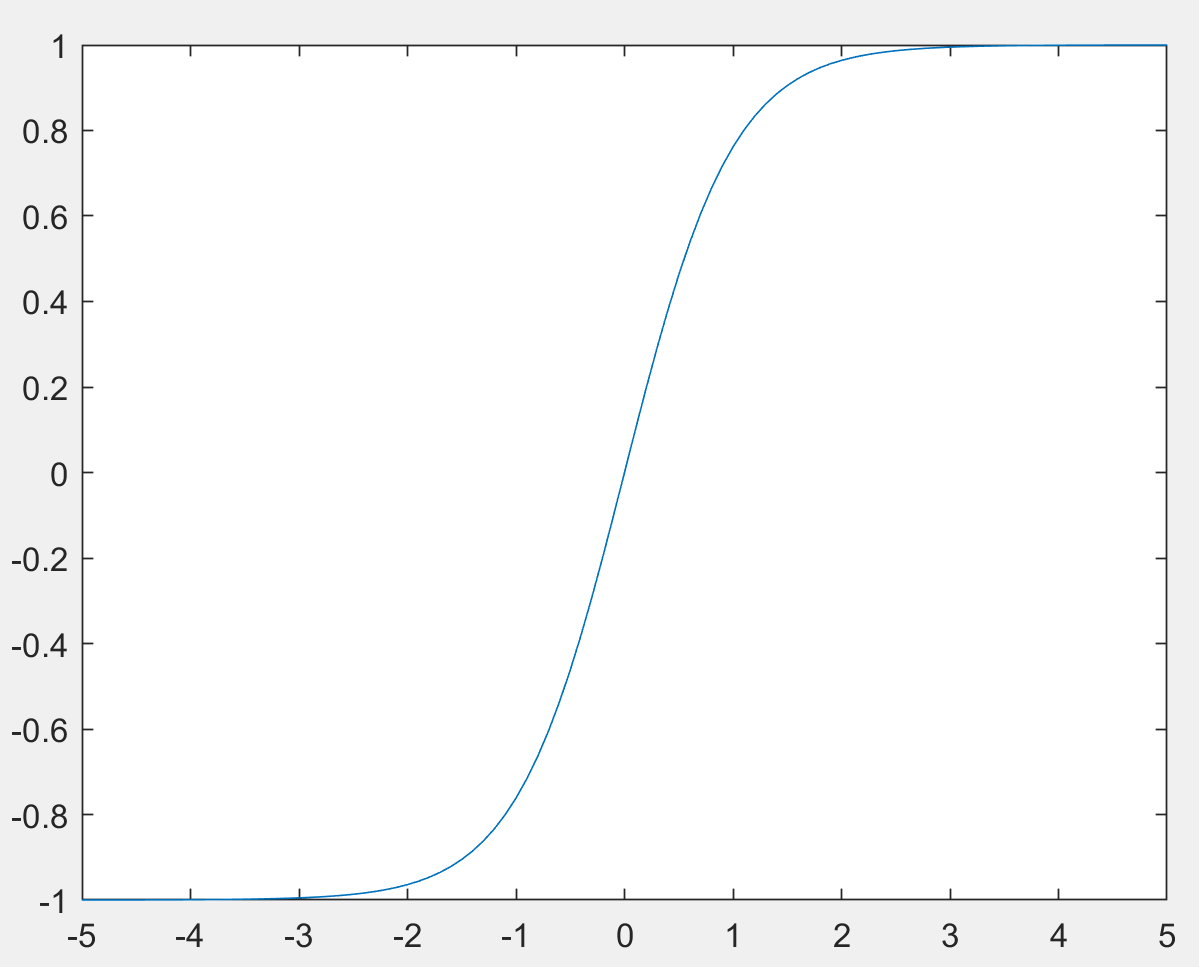
\includegraphics[width=0.4\textwidth]{Grafika/simgoidalna.png}
        \caption{Wykres funkcji sigmoidalnej wykonany przy pomocy Matlab R2019a}
        \label{fig:sigmoidalna}
    \end{figure}
    
    A także funkcja liniowa dla warstwy trzeciej:\\
    \begin{figure}[h]
        \centering
        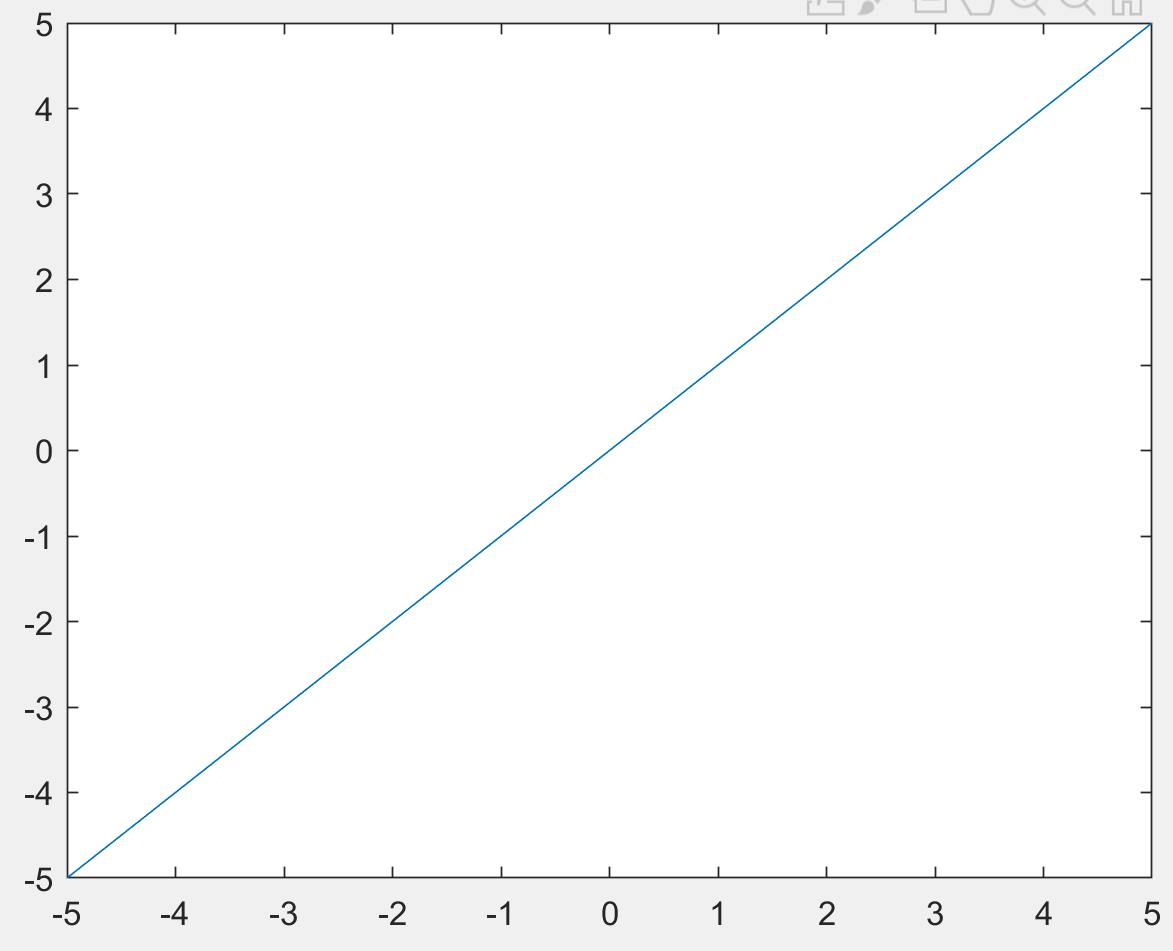
\includegraphics[width=0.4\textwidth]{Grafika/liniowa.png}
        \caption{Wykres funkcji liniowej wykonany przy pomocy Matlab R2019a}
        \label{fig:liniowa}
    \end{figure}\\
    Są to najczęściej wykorzystywane funkcje aktywacji. Są one zaimplementowane w Matlabie R2019a. Funkcja sigmoidalna posiada nazwę tansig, liniowa zaś purelin.
    
    \clearpage
    \subsection{Sieć neuronowa jednowarstwowa}
    Projekt zakłada wykorzystanie sieci wielowarstwowej. Omówienie sieci jednowarstwowej pozwoli jednak łatwiej zrozumieć koncepcje warstw uczenia, ponieważ jest ona elementem sieci wielowarstwowej.
    \begin{figure}[h]
        \centering
        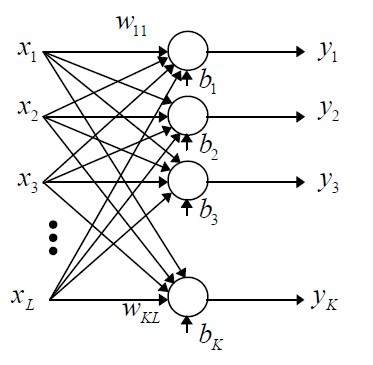
\includegraphics[width=0.5\textwidth]{Grafika/schemat_1w.jpg}
        \caption{Schemat sieci jednokierunkowej jednowarstwowej}
        \label{fig:SchematSieci1}
    \end{figure}\\
    Działanie sieci jednowarstwowej można opisać następująco
    \begin{equation} \label{dzialanie_jednowarstwowej}
    y = f\left(w x + b \right)
    \end{equation}
    gdzie:\\[0.3cm]
    $y = [y_1, y_2, ..., y_K]^T$  - wektor sygnałów wyjściowych \\[0.3cm]
    $x = [x_1,x_2,...,x_L]^T$ - wektor sygnałów wejściowych \\[0.3cm]
    $b = [b_1,b_2, ..., b_K]^T$ - wektor przesunięć \\[0.3cm]
    $w=\begin{bmatrix}
    w_{11} & w_{12} & w_{13} & \dots  & w_{1L} \\
    w_{21} & w_{22} & w_{23} & \dots  & w_{2L} \\
    \vdots & \vdots & \vdots & \ddots & \vdots \\
    w_{K1} & w_{K2} & w_{K3} & \dots  & w_{KL}
    \end{bmatrix}$ - macierz wag
    
    \\
    Proces uczenia ma za zadanie tak wybrać wagi, by z zadaną dokładnością odwzorować dane wejściowe w wyjściowe. Zmiana wag odbywa się w cyklach zwanych epokami. Dla j-tej wagi i-tego neuronu można to zapisać zależnością:
    \begin{equation} \label{zmiana_wag}
    w_{ij}(t+1) = w_{ij}(t) + \Delta w_{ij}(t)
    \end{equation}\\
    gdzie:\\[0.1cm]
    $t$ - numer cyklu
    \\[0.5cm]
    Rozważany w projekcie algorytm jest algorytmem uczenia z nauczycielem. Zatem każdemu wektorowi wejściowemu $x = [x_1,x_2,...,x_L]^T$ towarzyszy pożądany wektor sygnałów wyjściowych $\hat{y} = [\hat{y}_1,\hat{y}_2,...,\hat{y}_K]^T$. Para wektorów $(x,\hat{y})$ to para ucząca. Jeżeli sieć nie jest nauczona, to sygnał $\hat{y}$ różni się od sygnału wyjściowego $y$. Błąd popełniany przez sieć dla każdego wyjścia:
    \begin{equation} \label{error}
    e_i = y_i - \hat{y}_i
    \end{equation}
    W czasie uczenia dąży się do uzyskania zgodności $y$ z wartościami wymaganymi $\hat{y}$, Problem ten można sprowadzić do minimalizacji określonej funkcji celu. Przyjmując, że jest ona błędem średniokwadratowym wyznaczanym dla wszystkich $K$neuronów otrzymujemy:
    \begin{equation} \label{error2}
    E = \frac{1}{2} \sum^K_{i=1} e^2_i
    \end{equation}\\
    Ponieważ $E=E(w)$ minimum poszukiwać można metodą gradientową. Można to wykonać metodą największego spadku. Wektor wag przyrostu wyraża się następująco:
    \begin{equation} \label{gradient}
    \Delta  w = - \eta \nabla E(w)
    \end{equation}
    gdzie:\\[0.3cm]
    $\nabla$ - gradient,\\[0.1cm]
    $\eta$ - współczynnik uczenia.\\[0.3cm]
    Znak minus znajduje się we wzorze (\ref{gradient}) ponieważ gradient $\nabla E$ wskazuje kierunek najszybszego wzrostu funkcji, w minimalizacji chodzi zaś o kierunek odwrotny, czyli jak najszybszy spadek.\\
    Dla $i$-tego neuronu i $j$-tej wagi orzymujemy:\\
    \begin{equation} \label{gradient2}
    \Delta  w_{ij} = - \eta \frac{\partial E}{\partial w_{ij}}
    \end{equation}\\[0.3cm]
    Uwzględniając uwikłanie zależności $E$ od $w_{ij}$ poprzez $y_i$ i $n_i$, czyli $E = E(y_i(n_i(w_{ij})))$ pochodną możemy zapisać:\\
    \begin{equation}
    \label{eq:pochodna_gradient}
    \frac{\partial E}{\partial w_{ij}} = \frac{\partial E}{\partial y_i}  \frac{\partial y_i}{\partial n_i}  \frac{\partial n_i}{\partial w_{ij}}
    \end{equation}\\
    Uwzględniając zależności (\ref{error}) i (\ref{error2}) otrzymujemy:
    \begin{equation}
    \frac{\partial E}{\partial y_i} = y_i - \hat{y}_i = e_i
    \end{equation}
    Uwzględniając zależność (\ref{pobudzenieNeuronu}) otrzymujemy:
    \begin{equation}
    \frac{\partial n_i}{\partial w_{ij}} = x_j
    \end{equation}
    Wstawiając otrzymane pochodne do równania (\ref{eq:pochodna_gradient}), otrzymane równanie do zależności (\ref{gradient2}) otrzymujemy:
    \begin{equation}
        \label{gradient_podstawione}
        \Delta  w_{ij} = - \eta \frac{\partial E}{\partial w_{ij}} = \eta (\hat{y}_i - y_i) \frac{\partial y_i}{\partial n_i} x_j
    \end{equation}
    gdzie
    $\frac{\partial y_i}{\partial n_i} = f'(n_i)$ równe jest pochodnej cząstkowej $i$-tej funkcji aktywacji po $i$-tym łącznym pobudzeniu neuronu.
    
    \clearpage
    \subsection{Sieć neuronowa wielowarstwowa}
        \begin{figure}[h]
        \centering
        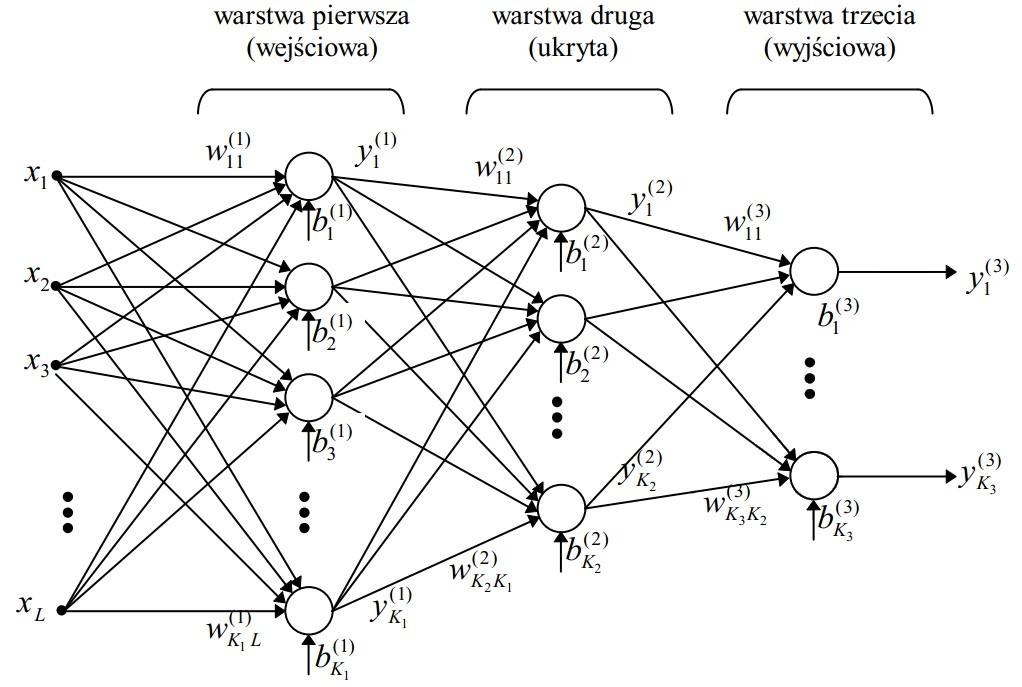
\includegraphics[width=0.8\textwidth]{Grafika/schemat_sieci.jpg}
        \caption{Schemat sieci jednokierunkowej wielowarstwowej}
        \label{fig:SchematSieci}
    \end{figure}\\
    Sieci jednokierunkowe składają się z neuronów przesyłających sygnały do kolejnych warstw:
    Z warstwy wejściowej do warstw ukrytych, z warstw ukrytych do warwowy wyjściowej.\\
    Na rysunku (\ref{fig:SchematSieci}) przedstawiono sieć trójwarstwową. Sygnały wejściowe warstwy są sygnałami wyjściowymi warstwy poprzedniej. Pomiędzy warstwami neuronów zastosowane są połączenia jeden do wielu. \\
    Warstwy posiadają swoją macierz wag (w), wektor przesunięć (b), funkcję aktywacji (f) a także sygnał wyjściowy (y). Do zapisów dodano numery warstw: np. zapis $w^{(3)} $ oznacza macierz wag trzeciej warstwy.\\
    Sposób działania poszczególnych warstw można opisać następująco:
     \begin{equation}
        \begin{aligned}
        y^{(1)} &= f^{(1)}(w^{(1)}x+b^{(1)})\\
        y^{(2)} &= f^{(2)}(w^{(2)}y^{(1)}+b^{(2)})\\
        y^{(3)} &= f^{(3)}(w^{(3)}y^{(2)}+b^{(3)})\\
        \end{aligned}    
    \end{equation}\\[0.3cm]
    Działanie sieci to więc:
    \begin{equation}
    y^{(3)} = f^{(3)}\Bigg(w^{(3)}f^{(2)}\bigg(w^{(2)}f^{(1)}\Big(w^{(1)}x+b^{(1)}\Big)+b^{(2)}\bigg)+b^{(3)}\Bigg)
    \end{equation}
    
    \clearpage
    \subsection{Wsteczna propagacja błędu}
    Wsteczna propagacja błędu jest mechanizmem służącym uczeniu sieci neuronowej. Polega na zaktualizowaniu wartości wag oraz przesunięć dla każdego neuronu, zaczynając od warstw wyższych, kierując się w stronę niższych.\\
    Dla sieci trójwarstwowej opisywana jest następująco:
    \\[0.2cm]
\begin{equation}
\begin{aligned}
    &E = \frac{1}{2} \sum_{i_{3}=1}^{K_3}e^{2}_{i_3} = \frac{1}{2}  \sum_{i_{3}=1}^{K_3}
    \Big(y^{(3)}_{i_3}-\hat y_{i_3}
    \Big)^{2} = \\
    &=\frac{1}{2}  \sum_{i_{3}=1}^{K_3}
    \Bigg( f^{(3)} 
    \Bigg(  \sum_{i_{2}=1}^{K_2}w^{(3)}_{i_3 i_2}y_{i_2}+b^{(3)}_{i_3}
    \Bigg)  -\hat y_{i_3}
    \Bigg)^{2} = \\
    &=\frac{1}{2}  \sum_{i_{3}=1}^{K_3}
    \Bigg( f^{(3)} 
    \Bigg( \sum_{i_{2}=1}^{K_2}w^{(3)}_{i_3 i_2} f^{(2)} 
    \Bigg( \sum_{i_{1}=1}^{K_1}w^{(2)}_{i_2 i_1} y_{i_1}+b^{(2)}_{i_2}
    \Bigg) +b^{(3)}_{i_3} 
    \Bigg) -\hat y_{i_3}
    \Bigg)^{2} = \\
    &=\frac{1}{2}  \sum_{i_{3}=1}^{K_3}
    \Bigg( f^{(3)} 
    \Bigg( \sum_{i_{2}=1}^{K_2}w^{(3)}_{i_3 i_2} f^{(2)}
    \Bigg( \sum_{i_{1}=1}^{K_1}w^{(2)}_{i_2 i_1} f^{(1)}
    \Bigg( \sum_{j=1}^{L}w^{(1)}_{i_1 j}x_{j} + b^{(1)}_{i_1}
    \Bigg) +b^{(2)}_{i_2}
    \Bigg) +b^{(3)}_{i_3} 
    \Bigg) -\hat y_{i_3}
    \Bigg)^{2}
\end{aligned}
\end{equation}\\

    Wyliczanie wag rozpoczyna się od wyliczenia wag neuronów warstwy wyjściowej. Na podstawie tych obliczeń obliczane są wagi warstwy wcześniejszej o jeden itd.\\[0.5cm]
    Dla drugiej warstwy sieci z rysunku (\ref{fig:SchematSieci}) otrzymujemy:\\[0.2cm]
    \begin{equation}
    \frac{\partial E}{\partial w^{(2)}_{i_2i_1}} = \sum_{i_{3}=1}^{K_3}\Big(e_{i_3} f'^{(3)}(n_{i_3}) w^{(3)}_{i_3 i_2}\Big)
    f'^{(2)}(n_{i_2}) y^{(1)}_{i_1}
    \end{equation}\\[0.2cm]
    Dla warstwy pierwszej otrzymujemy:\\[0.2cm]
    \begin{equation}
     \frac{\partial E}{\partial w^{(1)}_{i_1j}} = f'^{(1)}(n_{i_1}) x_j 
    \sum_{i_{2}=1}^{K_2}\Bigg( f'^{(2)}(n_{i_2}) w^{(2)}_{i_2 i_1}
     \sum_{i_{3}=1}^{K_3}\bigg(e_{i_3} f'^{(3)}(n_{i_3}) w^{(3)}_{i_3 i_2}   \bigg)\Bigg)
    \end{equation}

    \clearpage
    \subsection{Adaptacyjny współczynnik uczenia}
    Jest to metoda pozwalająca na przyspieszenie procesu uczenia. Polega na zmienianiu współczynnika uczenia $\eta$ w zależności od błędu popełnianego przez sieć.\\ 
    W metodzie tej błąd najczęściej wyraża się w postaci sumarycznego błędu kwadratowego $SSE$:
     \begin{equation}
        SSE(t)=\sum_{i=1}^M\bigg(y_i(t)-\hat{y}_i(t)\bigg)^2
    \end{equation}\\[0.1cm]
    bądź błędu średniokwadratowego $MSE$:
    \begin{equation}
         MSE(t)=\frac{1}{M}\sum_{i=1}^M\bigg(y_i(t)-\hat{y}_i(t)\bigg)^2
    \end{equation}\\[0.2cm]
    
    Zaktualizowanie współczynnika uczenia w czasie t+1 przedstawia się wzorem:
    \begin{equation}
        \eta(t+1)=\begin{cases}
            \eta(t) \cdot\xi _d \qquad \qquad gdy\quad ERR(t)>er\cdot ERR(t-1)\\
            \eta(t) \cdot\xi _i \qquad \qquad gdy\quad ERR(t)<ERR(t-1)\\
            \eta(t) \qquad \quad \qquad gdy\quad ERR(t-1) \leq ERR(t)\leq er\cdot ERR(t-1)\\
        \end{cases}
    \end{equation}\\[0.2cm]
     gdzie:\\[0.3cm]
     $\eta$ - współczynnik uczenia\\
     $\xi _d$ - współczynnik zmniejszania $\eta$\\
     $\xi _i$ - współczynnik zwiększania $\eta$\\
     $er$ - dopuszczalny błąd sieci\\
     $ERR$ - wartość błędu $SSE$ bądź $MSE$\\[0.5cm]
     
     
    Gdy nowy błąd jest istotnie większy od poprzedniego - współczynnik jest zmniejszany.\\
    W przypadku gdy nowy błąd jest istotnie mniejszy – współczynnik jest zwiększany.\\
    Jeżeli błąd w kroku k zwiększył się w porownaniu do błędu z kroku k-1, ale nie w sposób istotny (4\% dla wartości $er$ równej 1.04) - współczynnik nie zmienia się.
    
    \clearpage
    \section{Skrypt}
    Skrypt wykorzystany do realizacji projektu został zrealizowany przy pomocy programu Matlab w wersji R2019a. Implementując adaptacyjny współczynnik uczenia posłużono się sumarycznym błędem kwadratowym SSE. Poniżej przedstawiony został kod na którym bazowały przeprowadzone eksperymenty. Był on modyfikowany w zależności od potrzeb danego eksperymentu.
    
    \begin{lstlisting}[language=Matlab, caption=Skrypt użytej sieci neuronowej, label=skrypt,numbers=left]
clear;
close all;
clc;
format compact;
	 
DValue = importdata('glass.data', ',');
Value2=DValue(:,2:10);
y2 = DValue(:,11);
	 
 
Pn = Value2;
T = y2;
 
Pn = transpose(Pn);
T = transpose(T);
	 
Pn = mapminmax(Pn);
T=mapminmax(T);
 
trainFcn = 'traingda';  
 
S1_vec = 1:1:20;
S2_vec = S1_vec;
 
PK_v=zeros (length(S1_vec),length(S2_vec));
	SSE_v=PK_v;
 
 
for S1 = S1_vec
    for S2 = S2_vec:S1 
        for ind_lr_inc=1:length(lr_inc_vec)
            for ind_lr_dec=1:length(lr_dec_vec)
                for ind_e=1:length(e_vec)
                    % Create a Pattern Recognition Network
        	        hiddenLayerSize = [S1,S2];
        	        net = feedforwardnet(hiddenLayerSize, trainFcn);
        	        net.performFcn = 'sse';
        	        net.layers{1}.transferFcn='tansig';
        	        net.layers{2}.transferFcn='tansig';
        	        net.layers{3}.transferFcn='purelin';
        	 
        	        net.trainParam.epochs = 10000;
        	        net.trainParam.max_fail = 50;
        	        net.trainParam.lr = 0.01;
        	        net.divideFcn = 'dividetrain';
        	        net.trainParam.goal = 0.25;
        	                                       
        	        % Train the Network
        	        [net,tr] = train(net,Pn,T);
        	        % Test the Network
        	        y = net(Pn);
        	        e = gsubtract(T,y);
        	        performance = perform(net,T,y);
        	                           
        	   
        	        PK = (1-sum(abs(T-y)>=1 )/length(T))*100
        	                                   
        	        PK_v(S1, S2) = PK;
                    SSE_v(S1, S2) = tr.best_perf;
                end
             end
        end
    end
end
% View the Network
view(net)
	 
save("output8.mat")
    \end{lstlisting}
    
    
\clearpage
\section{Eksperymenty}
\subsection{Eksperyment 1.}
    Eksperyment miał za zadanie sprawdzić z grubsza ilość neuronów potrzebnych do rozwiązania zadania. Zastosowane parametry:
    
    \begin{itemize}
        \item Neurony w warstwach: od 1 do 67 z krokiem co 5
        \item Pozostałe wartości domyślne dla funkcji $traingda$
       \end{itemize}
       
        \begin{figure}[!h]
            \centering
            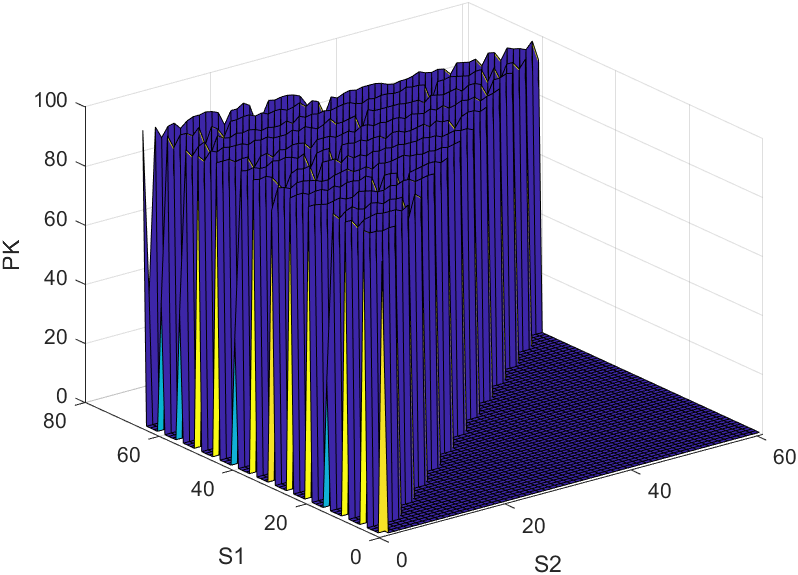
\includegraphics[width = 0.6\textwidth]{Grafika/eksperymenty/pk1.png}
            \caption {Wykres zależności PK od ilości neuronów w warstwacch dla Eksperymentu 1.}
            \label{fig:PKeksperyment1}
        \end{figure}
        \begin{figure}[!h]
            \centering
            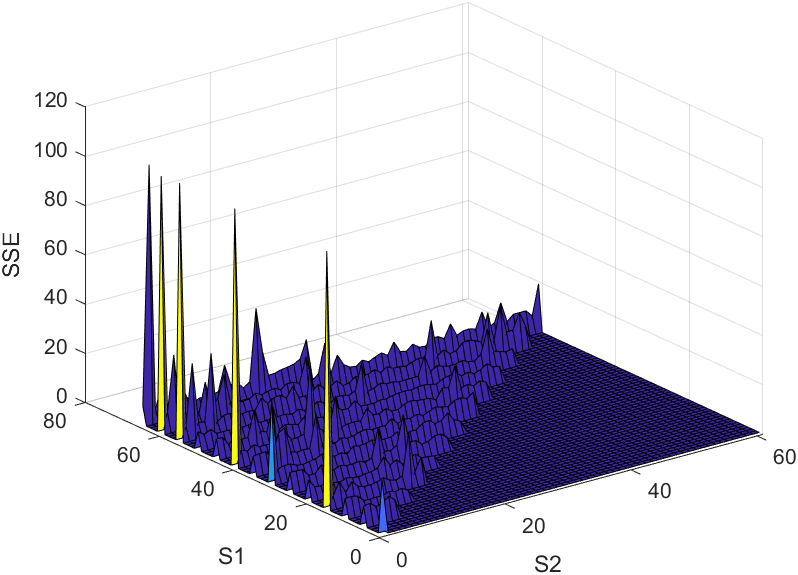
\includegraphics[width = 0.6\textwidth]{Grafika/eksperymenty/sse1.png}
            \caption {Wykres zależności SSE od ilości neuronów w warstwach dla Eksperymentu 1.}
            \label{fig:PKeksperyment1}
        \end{figure}
    Sieć już dla małych ilości neuronów potrafi osiągnąć zadowalające wartości PK oscylujące w granicach 90\%. Obserwując wykres błędu możemy zaobserwować pojedyncze ekstremalnie wysokie wartości spowodowane czynnikami losowymi. Pozostałe wartości SSE mieszczą się w granicach zbioru <2;10>.
    \clearpage
    \subsection{Eksperyment 2.}
    Eksperyment ten miał za zadanie dokładnie wyznaczyć najlepszą ilość neuronów w warstwach. Dobierając parametry wyciągnięto wnioski z poprzedniego eksperymentu.
      \begin{itemize}
        \item Neurony w warstwach: od 1 do 20 z krokiem co 1
        \item Pozostałe wartości domyślne dla funkcji $traingda$
       \end{itemize}
         \begin{figure}[!h]
            \centering
            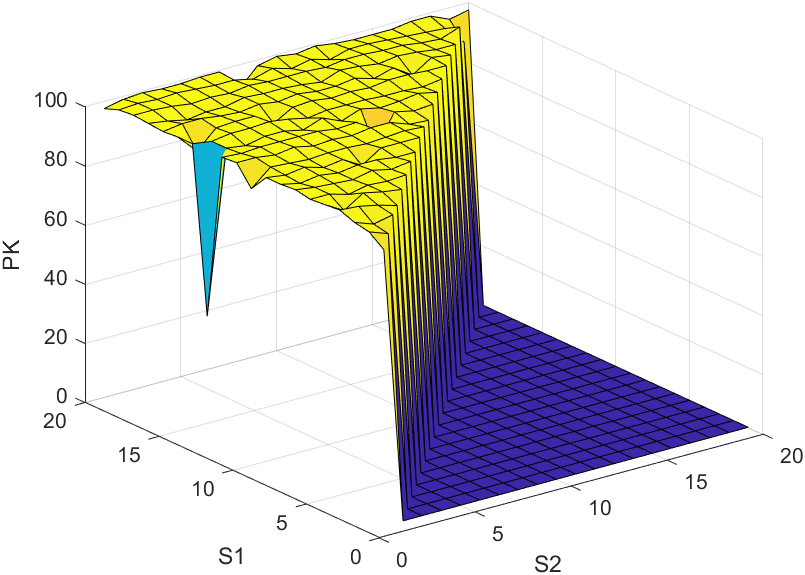
\includegraphics[width = 0.6\textwidth]{Grafika/eksperymenty/pk2.png}
            \caption {Wykres zależności PK od ilości neuronów w warstwach dla Eksperymentu 2.}
            \label{fig:PKeksperyment2}
        \end{figure}
        \begin{figure}[!h]
            \centering
            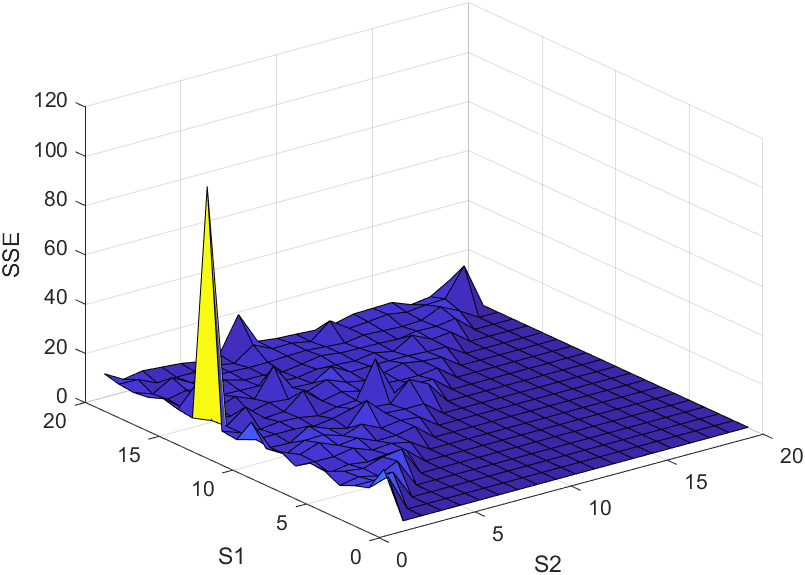
\includegraphics[width = 0.6\textwidth]{Grafika/eksperymenty/sse2.png}
            \caption {Wykres zależności SSE od ilości neuronów w warstwach dla Eksperymentu 2.}
            \label{fig:PKeksperyment2}
        \end{figure}   
        
        Analizując wykresy można dojść do identycznych wniosków z wnioskami Eksperymentu 1. Dla każdej z testowanych konfiguracji wartość PK była zbliżona do 100\%. Błąd zawierał się w przedziale o identycznym poziomie wielkości do poprzedniego eksperymentu.
    \clearpage    
    \subsection{Eksperyment 3.}
    Eksperyment miał za zadanie sprawdzić wpływ wartości zwiększania, a także zmniejszania współczynnika uczenia. By tego dokonać wybrano wartość neuronów w warstwach dla którego osiągnięto powyżej 99\% wartości PK.
     \begin{itemize}
        \item S1: 7 neuronów
        \item S2: 2 neurony
        \item lr\textunderscore inc: wartości od 1 do 1.09 z krokiem 0.01
        \item lr\textunderscore dec: wartości od 0.5 do 0.9 z krokiem 0.1
       \end{itemize}
       \begin{figure}[!h]
            \centering
            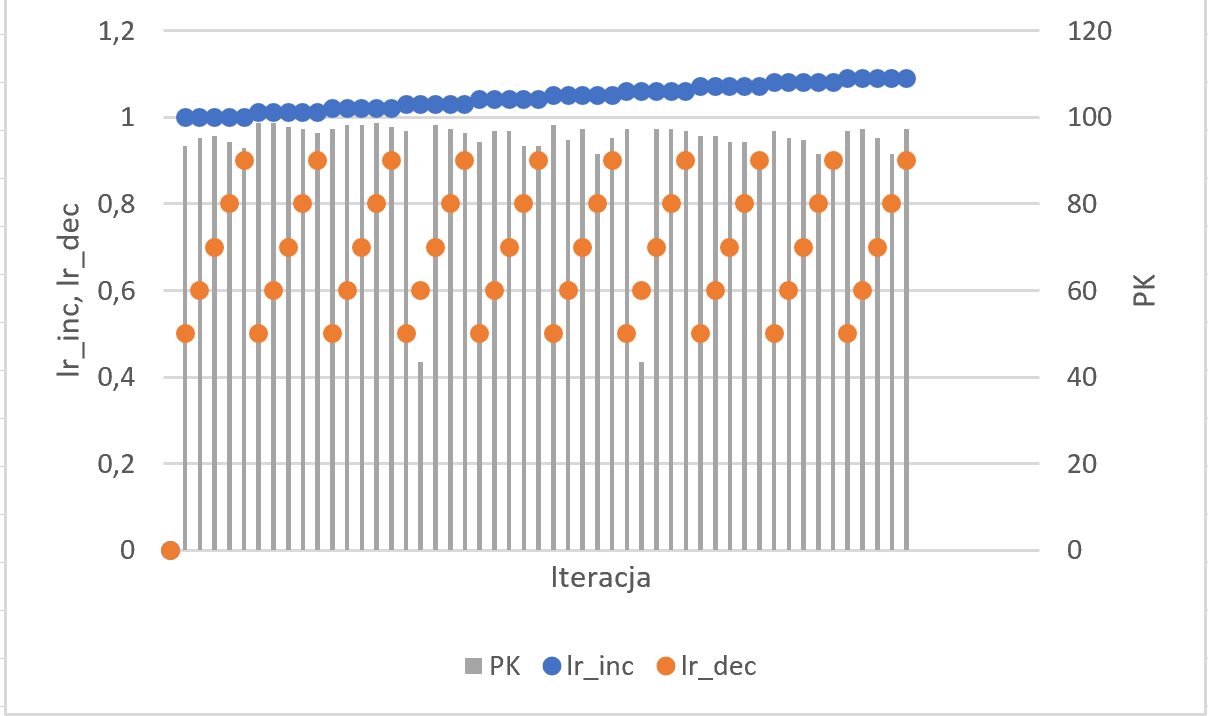
\includegraphics[width = 0.6\textwidth]{Grafika/eksperymenty/pk3.png}
            \caption {Wykres zależności PK od ilości wartości zmniejszania i zwiększania współczynnika uczenia dla Eksperymentu 3.}
            \label{fig:PKeksperyment3}
        \end{figure}
        \begin{figure}[!h]
            \centering
            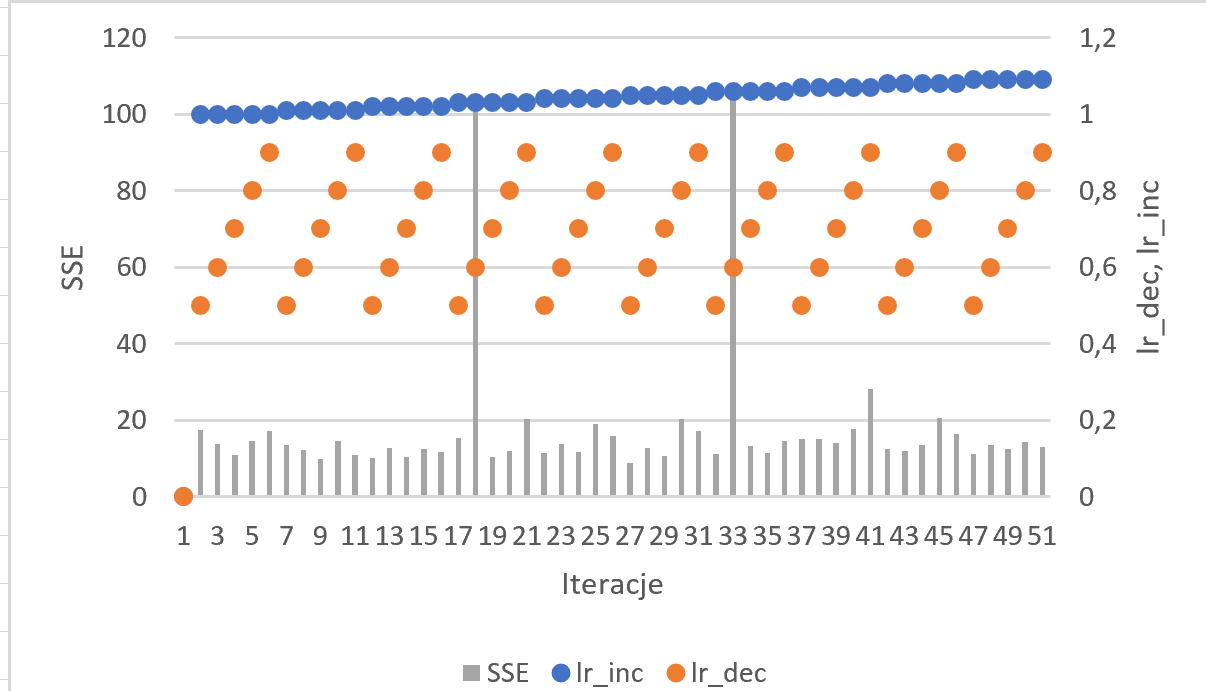
\includegraphics[width = 0.6\textwidth]{Grafika/eksperymenty/sse3.png}
            \caption {Wykres zależności SSE od ilości wartości zmniejszania i zwiększania współczynnika uczenia dla Eksperymentu 3.}
            \label{fig:PKeksperyment3}
        \end{figure}   
        Interpretując wykresy możemy możemy zauważyć, że współczynniki inkrementacji i dekrementacji współczynnika uczenia nie mają wielkiego wpływu na poprawność klasyfikacji i błąd SSE. Najlepsza osiągnięta wartość PK wynosi 98,59813084, dla parametrów lr\textunderscoreinc = 1.02, lr\textunderscoredec = 0.8. Wartość SSE dla tych wartości to 12,35845925.\\
        Najniższy osiągnięty błąd to z kolei 8,915806587 dla pary 1.05, 0.5. Wartość PK dla tych wartości współczynników zmiany wartości współczynnika uczenia jest bliska optymalnemu, wynosi bowiem 98,13084112.
    
    \clearpage
    \subsection{Eksperyment 4.}
    Eksperyment miał na celu sprawdzenie, czy zwiększenie maksymalnej liczby epok pozytywnie wpłynie na wartość sumy błędu kwadratowego.
    \begin{itemize}
        \item Maksymalna liczba epok: 50000
        \item Neurony w warstwach: od 2 do 8 z krokiem co 1
        \item Pozostałe wartości domyślne dla funkcji $traingda$
    \end{itemize}
        \begin{figure}[!h]
            \centering
            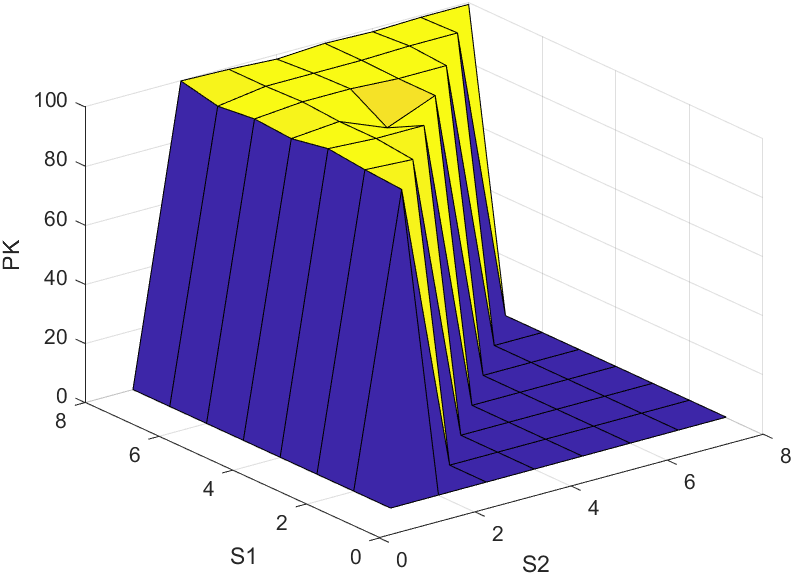
\includegraphics[width = 0.6\textwidth]{Grafika/eksperymenty/pk4.png}
            \caption {Wykres zależności PK od ilości neuronów w warstwach dla Eksperymentu 4.}
            \label{fig:PKeksperyment4}
        \end{figure}
        \begin{figure}[!h]
            \centering
            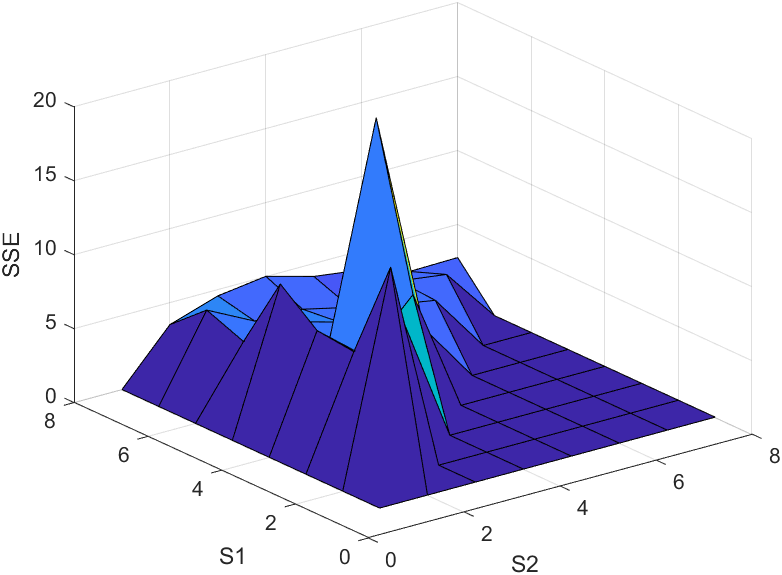
\includegraphics[width = 0.6\textwidth]{Grafika/eksperymenty/sse4.png}
            \caption {Wykres zależności SSE od ilości neuronów w warstwach dla Eksperymentu 4.}
            \label{fig:PKeksperyment4}
        \end{figure}   
        Po pięciokrotnym zwiększeniu liczby epok udało się uniknąć ekstremalnych skoków wartości SSE obserwowalnych w poprzednich eksperymentach, spowodowanych czynnikami losowami, jednak statystycznie rząd wielkości wartości SSE pozostał na tym samym poziomie.\\
        Najlepszymi epokami, były epoki zbliżone do 50000 (wartości z przedziału 49944 – 49999).
        
        \clearpage
        \subsection{Eksperyment 5.}
        Eksperyment ten miał na celu sprawdzenie wpływu dopuszczalnego błędu sieci na proces uczenia.
        \begin{itemize}
            \item S1: 7 neuronów
            \item S2: 2 neurony
            \item Dopuszczalny błąd sieci: wartości od 1 do 2 z krokiem 0.01
            \item ir\textunderscore inc: 1.05
            \item lr\textunderscore dec: 0.7
        \end{itemize}
         \begin{figure}[!h]
            \centering
            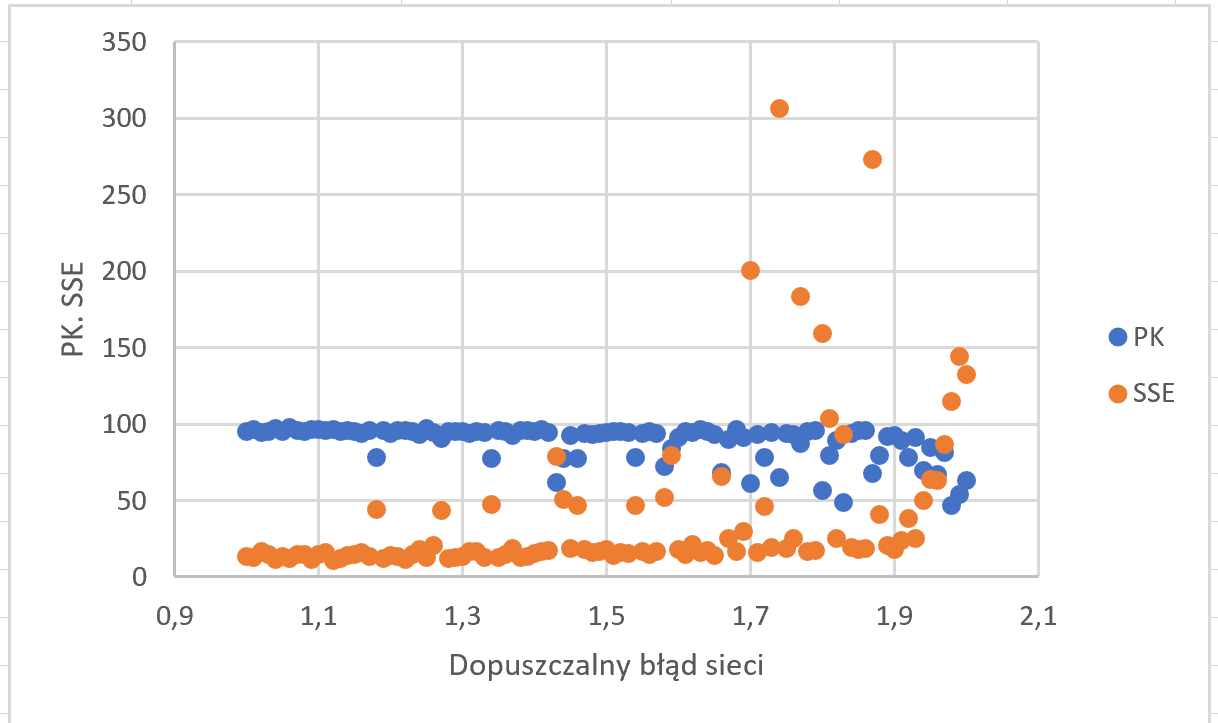
\includegraphics[width = 0.6\textwidth]{Grafika/eksperymenty/pksse5.png}
            \caption {Wykres zależności PK i SSE od dopuszczalnego błędu sieci}
            \label{fig:PSSEKeksperyment5}
        \end{figure}
        Analizując wykres możemy zaobserwować, że od wartości 1 do 1,7 nie występują poważne odchylenia SSE. Po przekroczeniu wartości 1.7 są one coraz częstsze, a po przekroczeniu 1.9 SSE rośnie liniowo.
        
        \clearpage
        \section{Wnioski}
        Celem projektu było rozpoznawanie rodzaju naczyń szklanych skryptem sieci neuronowej uczonej algorytmem wstecznej propagacji błędu z adaptacyjnym współczynnikiem uczenia. Udało się spełnić założenia projektu, a także zapoznać się z tym tematem\\
    Część praktyczna projektu została wykonana w programie Matlab, który posiada zaimplementowane wszystkie niezbędne do wykonania ćwiczenia funkcje. Przede wszystkim warto wymienić funkcję traingda, która zastąpiła znaną z poprzednich wersji funkcję trainbpa. Odpowiednie jej użycie pozwoliło na przeprowadzenie wszystkich eksperymentów. Użyto również funkcji do rysowania wykresów, a także importowania tabel do programu Excel.\\
    Dzięki przeprowadzonym eksperymentom udało się zaobserwować jak wartości poszczególnych parametrów uczenia wpływają na jego rezultat.\\
    Wykonanie projektu dowiodło również, że praca z sieciami neuronowymi wymaga dużej ilości czasu, mocy obliczeniowych komputera, a także wyczucia i doświadczenia w wybieraniu parametrów uczenia.\\[1cm]


 \begin{thebibliography}{9}

\bibitem{mathworks}
\url{http://archive.ics.uci.edu/ml/datasets/Glass+Identification}

\bibitem{neuron} 
dr hab. inż. Roman Zajdel. 
\textit{Sztuczna inteligencja, Laboratorium, Ćw6 Model neuronu}. 

\bibitem{siec_jednowarstwowa} 
dr hab. inż. Roman Zajdel. 
\textit{Sztuczna inteligencja, Laboratorium, Ćw8 Sieć jednokierunkowa jednowarstwowa}. 

\bibitem{siec_wielowarstwowa} 
dr hab. inż. Roman Zajdel. 
\textit{Sztuczna inteligencja, Laboratorium, Ćw9 Sieć jednokierunkowa wielowarstwowa}.

\bibitem{momentum} 
dr hab. inż. Roman Zajdel. 
\textit{Sztuczna inteligencja, Laboratorium, Ćw10 Przyśpieszanie procesu uczenia}.

\bibitem{Kluska} 
prof. dr hab. inż. Jacek Kluska. 
\textit{Wykłady ze sztucznej inteligencji}.

\bibitem{book} 
L. Rutkowski
\textit{Metody i techniki sztucznej inteligencji, Wydawnictwo Naukowe PWN, Warszawa 2019}

\bibitem{mathworks}
\url{https://www.mathworks.com/help/deeplearning/ref/traingda.html}

\bibitem{mathworks}
\url{http://pl.wikipedia.org/wiki/Sieć_neuronowa}

\end{thebibliography}
    \end{document}